\setlength{\footskip}{8mm}

\chapter{LITERATURE REVIEW}

Write your introductory paragraph/s to give an overview of the chapter (except for Chapter 1). Limit this section to two paragraphs. Follow the appropriate structure of writing paragraphs. Paragraphs should have at least four sentences (8 lines). Paragraphs with more than 6 sentences (12 lines) must be split into two paragraphs.  Maintain one blank line between paragraphs.

\section{Measuring Glucose in blood}

Measured Raman signal can be seen as four parts \cite{directGlucose}. 
(1) glucose Raman spectrum (G), (2) tissue (non-glucose) Raman spectrum (T), (3) time-varying tissue background signal ($B_T$), and (4) time-independent system background signal ($B_S$).
Glucose signals changes according to the amount of glucose that exists in the blood. 
This means $\Delta G = G_{t_1} - G_{t_2}$ where $G_{t_1}$ and $G_{t_2}$ is glucose signal at time $t_1$ and $t_2$ respectively.
Tissue Raman is generated by lipids, proteins, and collagen. 
When measuring the same spot, the tissue Raman stays relatively unchanged.
This means $\Delta T = T_{t_1} - T_{t_2} \approx 0$.
For time-varying tissue background and time-independent system background, the difference at two-time points is $\Delta B_T = B_{T_{t_1}} - B_{T_{t_2}}$ and $\Delta B_S = B_{S_{t_1}} - B_{S_{t_2}}$.
Given the $\Delta t$ is small, $\Delta B_T$ and $\Delta B_S$ is $\approx 0$.

The Raman signal ($R$) consists of four parts that can be modeled as $R = G + T + B_T + B_S$.
Then, the $\Delta R$ would be $\Delta G + \Delta T + \Delta B_T + \Delta B_S$.
It is obvious that, given $\Delta t$ is small, the $\Delta R = \Delta G + 0 + 0 + 0 = G_{t_1} - G_{t_2}$.




%%%%%%%%%%%%%%%%%%%%%%%%%%%%%
\section{Glucose fingerprint}

\begin{figure}
    \caption{Raman spectra of (A) galactose and (B) glucose, both crystalline. 
    $\lambda_{ex}$ 532 nm, $P$ 20 mW, $t_{\text{ac}}$ 2 min \citep{crystallineGlucose}}
    \centerline{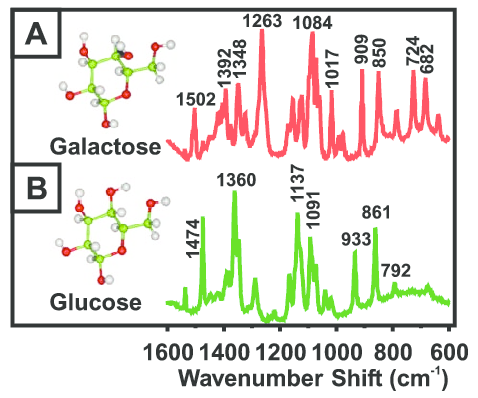
\includegraphics[width=3in]{figures/crytallineGlucose-RS.png}}
    \label{fig:crytallineGlucose-RS}
    % \small{\textit{Note.} Additional notes goes here.}
\end{figure}

Figure~\ref{fig:crytallineGlucose-RS} shows the direct measurement Raman scattering of crystalline glucose using 20 mW 532 nm laser \citep{crystallineGlucose}.
The numbers indicate in the figure are the signature peaks of glucose in crystalline form. The number are 792, 861, 933, 1091, 1137, 1360, and 1474 $\text{cm}^{-1}$.

\begin{figure}
    \caption{Raman spectra of glucose solution at different concentration \citep{solutionGlucose}.}
    \centerline{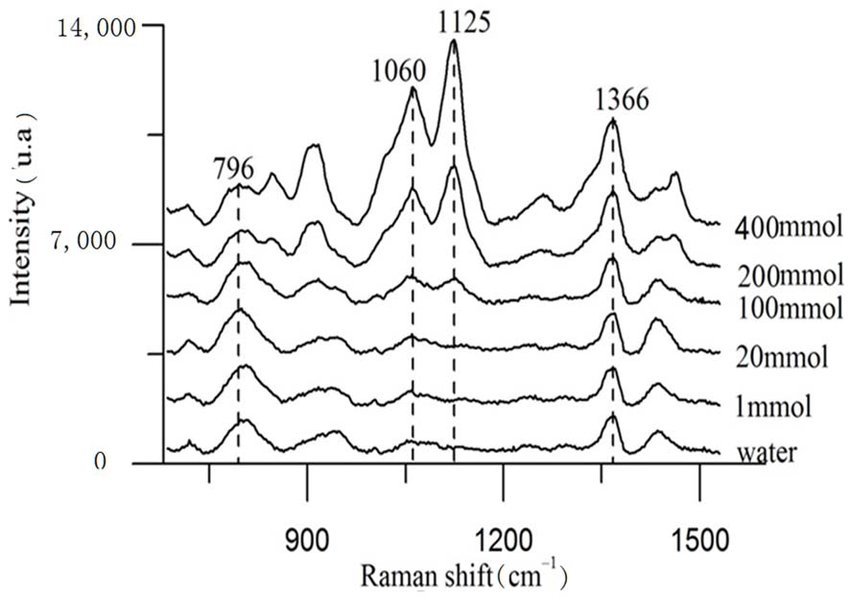
\includegraphics[width=3in]{figures/solutionGlucose-RS.jpg}}
    \label{fig:solutionGlucose-RS}
    % \small{\textit{Note.} Additional notes goes here.}
\end{figure}

Figure~\ref{fig:solutionGlucose-RS} shows the Raman shift of glucose solution at different concentrations.
Here, the peaks are 796, 1060, 1142, and 1366 $\text{cm}^{-1}$.
Comparing the peaks of the two glucose form, the wavenumber of peaks are close but the height is not.

\begin{figure}
    \caption{Raman spectra of lyophilized glucose compare with blood glucose measure at wrist \citep{sitecompare}.}
    \centerline{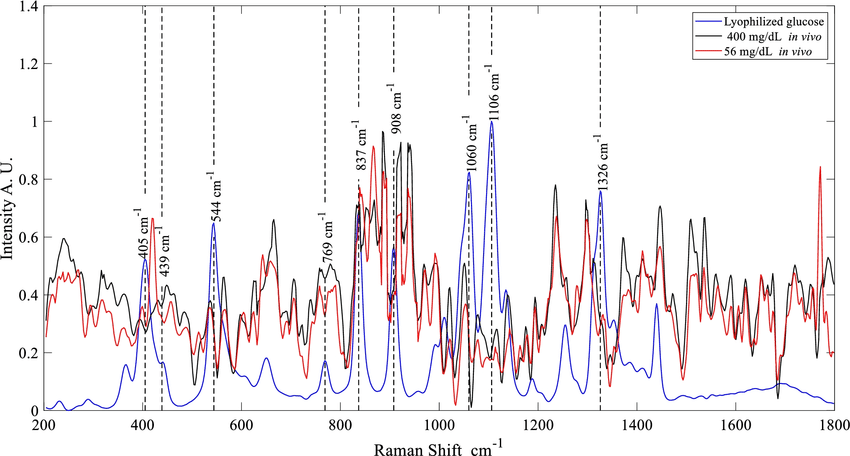
\includegraphics[width=3in]{figures/lyophilizedGlucose-RS.png}}
    \label{fig:lyophilizedGlucose-RS}
    % \small{\textit{Note.} Additional notes goes here.}
\end{figure}

\cite{sitecompare} reported the peaks of lyophilized (Freeze-drying) glucose and compared with blood glucose measured from the wrist (Figure~\ref{fig:lyophilizedGlucose-RS}).
The reported peaks of lyophilized glucose are 405, 439, 544, 769, 837, 908, 1060, 1106, and 1326 $\text{cm}^{-1}$.
For the forearm peaks at 544, 837, and 1060 $\text{cm}^{-1}$.
For the wrist, the peaks at 544 and 837 $\text{cm}^{-1}$. 
And, the index finger at 544 and 837 $\text{cm}^{-1}$. 
Molecular vibrations per each peak are 544 $\text{cm}^{-1}$ exocyclic deformation \citep{exocyclicdeformation}, 
837 $\text{cm}^{-1}$ vibrations $\nu$(C–C) \citep{vibrationsc-c}, 
and 1060 $\text{cm}^{-1}$ stretching $\nu$(C-O) and $\nu$(C–C) \citep{stretchingc-oc-c, exocyclicdeformation}.

\begin{figure}
    \caption{(\textbf{A}) Raman spectra of blood glucose obtained by subtracting two Raman signals \citep{directGlucose}.}
    \centerline{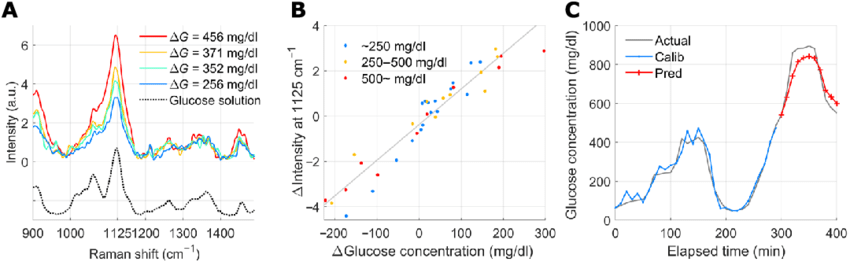
\includegraphics[width=3in]{figures/bloodGlucose-DeltaG.png}}
    \label{fig:bloodGlucose-DeltaG}
    % \small{\textit{Note.} Additional notes goes here.}
\end{figure}

\begin{figure}
    \caption{(\textbf{A}) Raman spectra of blood glucose measure at nailfold \citep{ramanNailFold2019}.}
    \centerline{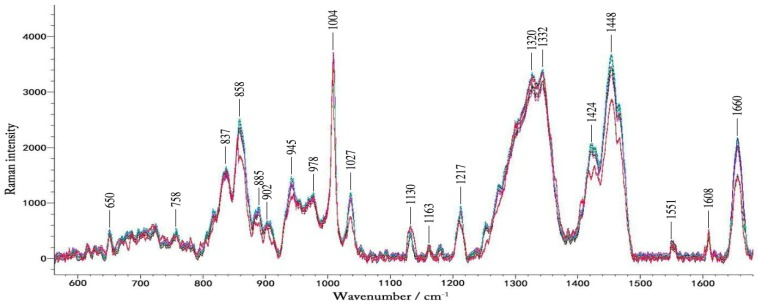
\includegraphics[width=3in]{figures/bloodGlucose-nailfold.jpg}}
    \label{fig:bloodGlucose-nailfold}
    % \small{\textit{Note.} Additional notes goes here.}
\end{figure}

For measuring glucose in the blood, \cite{directGlucose} showed the Raman shift obtained by subtracting the two Raman signals showed a significant peak at 1125 $\text{cm}^{-1}$ (Figure~\ref{fig:bloodGlucose-DeltaG}A).
Figure~\ref{fig:bloodGlucose-nailfold} shows the peaks number that agreed with the other works (837, 858, 945, 1027, 1130, and 1448 $\text{cm}^{-1}$). 
In addition, Table~\ref{tab:bloodpeak} shows what to expect when the Raman signal is measured correctly.

\begin{table}[]
    \caption{Assignments of Raman peaks that are identified in the spectra of the microvessels and blood \citep{peak45,forearm2005,peak47,peak48}}
    \begin{center}
    \begin{tabular}{cccc}
    \hline
    \multicolumn{2}{l}{Peak Position ($\text{cm}^{-1}$)} & \multirow{2}{*}{Assignments}  & \multirow{2}{*}{Components} \\ \cline{1-2}
    Microvessels         & Blood         &                               &                             \\ \cline{1-2}
    \hline
    650                  & 643           & P:C-S str                     & Ascorbic acid               \\
    758                  & 752           & $\nu_{15}$                    & Trp                         \\
    837                  & 827           & $\gamma10$                    & Fructose                    \\
    858                  & 855           & $\nu(C-C)$                    & Tyr, lac                    \\
    885                  & -             & -                             & -                           \\
    902                  & 898           & p:C-C skeletal                & Tyr                         \\
    945                  & 940           & $\nu(C-C)$                    & Crtic acid                  \\
    978                  & 971           & p: Skeletal vibr              & Fibrin                      \\
    1004                 & 1004          & $\nu$-ring                    & Phe                         \\
    1027                 & 1026          & $\delta(={C}_{b}{H}_{2})$asym & Lac                         \\
    1130                 & 1129          & $\nu_5$,                      & Lac                         \\
    1163                 & 1157          & $\nu_{44}$                    & Heme                        \\
    1217                 & 1212          & $\nu_5 + \nu_{18}$            & Heme                        \\
    1320                 & 1321          & p: CH2 twist                  & Try                         \\
    1332                 & 1341          & $\nu_{41}$                    & Trp                         \\
    1424                 & 1423          & $\nu_{28}$                    & Acetates                    \\
    1448                 & 1450          & $\delta(={CH}_{2}/{CH}_{3})$  & Trp                         \\
    1551                 & 1546          & $\nu_{11}$                    & Heme                        \\
    1608                 & 1603          & $\nu(C=C)_{\text{venyl}}$     & Heme                        \\
    1660                 & 1653          & Amide I                       & Heme                        \\
    \hline
    \end{tabular}
    \label{tab:bloodpeak}
    \end{center}
\end{table}



%%%%%%%%%%%%%%%%%%%%%%%%%%%%%%%%%
\section{Relationship of Raman scattering and glucose concentration}

\begin{figure}
    \caption{(\textbf{A}) Blood glucose value with 1125 $\text{cm}^{-1}$ relative intensity. (\textbf{B}) Concentration-dependent Raman relative intensities of glucose (1125 $\text{cm}^{-1}$) \citep{solutionGlucose}}
    \centerline{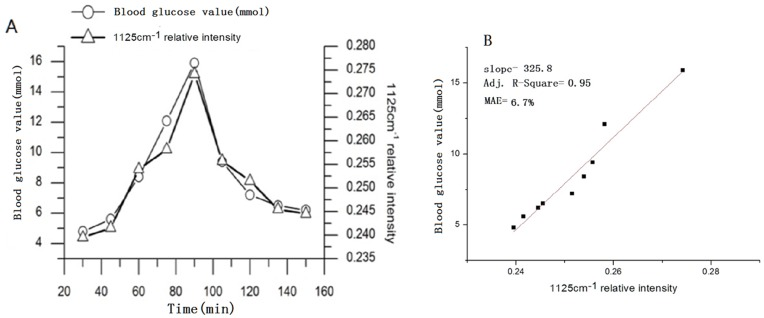
\includegraphics[width=3in]{figures/bloodGlucose-relative1125.png}}
    \label{fig:bloodGlucose-relative1125}
    % \small{\textit{Note.} Additional notes goes here.}
\end{figure}

In glucose solution, the concentration of 0.1 - 40 mmol/L of glucose in water and Raman shift at 1125 $\text{cm}^{-1}$ has a linear relationship \cite{solutionGlucose}.
The same case can not be said with blood glucose.
Since blood contains multiple components, using 1125 $\text{cm}^{-1}$ directly will not work. 
\cite{directGlucose} shows that the ratio of 1125 and 1450 (protein/lipid peak) $\text{cm}^{-1}$ yield a linear relationship.
Figure~\ref{fig:bloodGlucose-relative1125} shows that the normalized 1125 $\text{cm}^{-1}$ has a linear relationship with the glucose concentration.
This same procedure is also presented in \citep{solutionGlucose} where 1549 $\text{cm}^{-1}$ is used to normalize the spectrum.
On the other hand, \cite{ramanNailFold2019} uses PCA and BP-ANN with an input layer of 3, a hidden layer of 4, and an output layer of 1. 
While the model achieved an RMSE of 0.27 in intersubject modeling, using PCA is not necessarily means the features in use is a glucose-related feature \citep{directGlucose}.
Adding to the neural network, FFNN is primarily used in modeling glucose in \citep{sitecompare}. 
Without any feature selection, the RMSE of glucose prediction is 3.1 mmol/L and 30.12 mmol after implementing SOM and RReliefF as automatic feature selection.




%%%%%%%%%%%%%%%%%%%%%%%%%
\section{Concentration Limitation}

The usual blood glucose range of a healthy person can be as low as 0.3 - 1 mmol/L and $<$3 mmol/L for diabeties \citep{solutionGlucose}.

% \begin{equation}
%     y = mx+b
% \end{equation}

% \begin{table}[]
% \caption{An example table in latex.}
% \begin{center}
% \begin{tabular}{l l}
% \hline
%     Methods & Metric\\ \hline
% Method A      & 153.3                \\ 
% Method B & 2.4                  \\ \hline
% \end{tabular}
% \label{tab:dense}
% \end{center}
% \small{\textit{Note.} Add notes here.}
% \end{table}
